% Created by tikzDevice version 0.10.1 on 2017-04-09 19:11:13
% !TEX encoding = UTF-8 Unicode
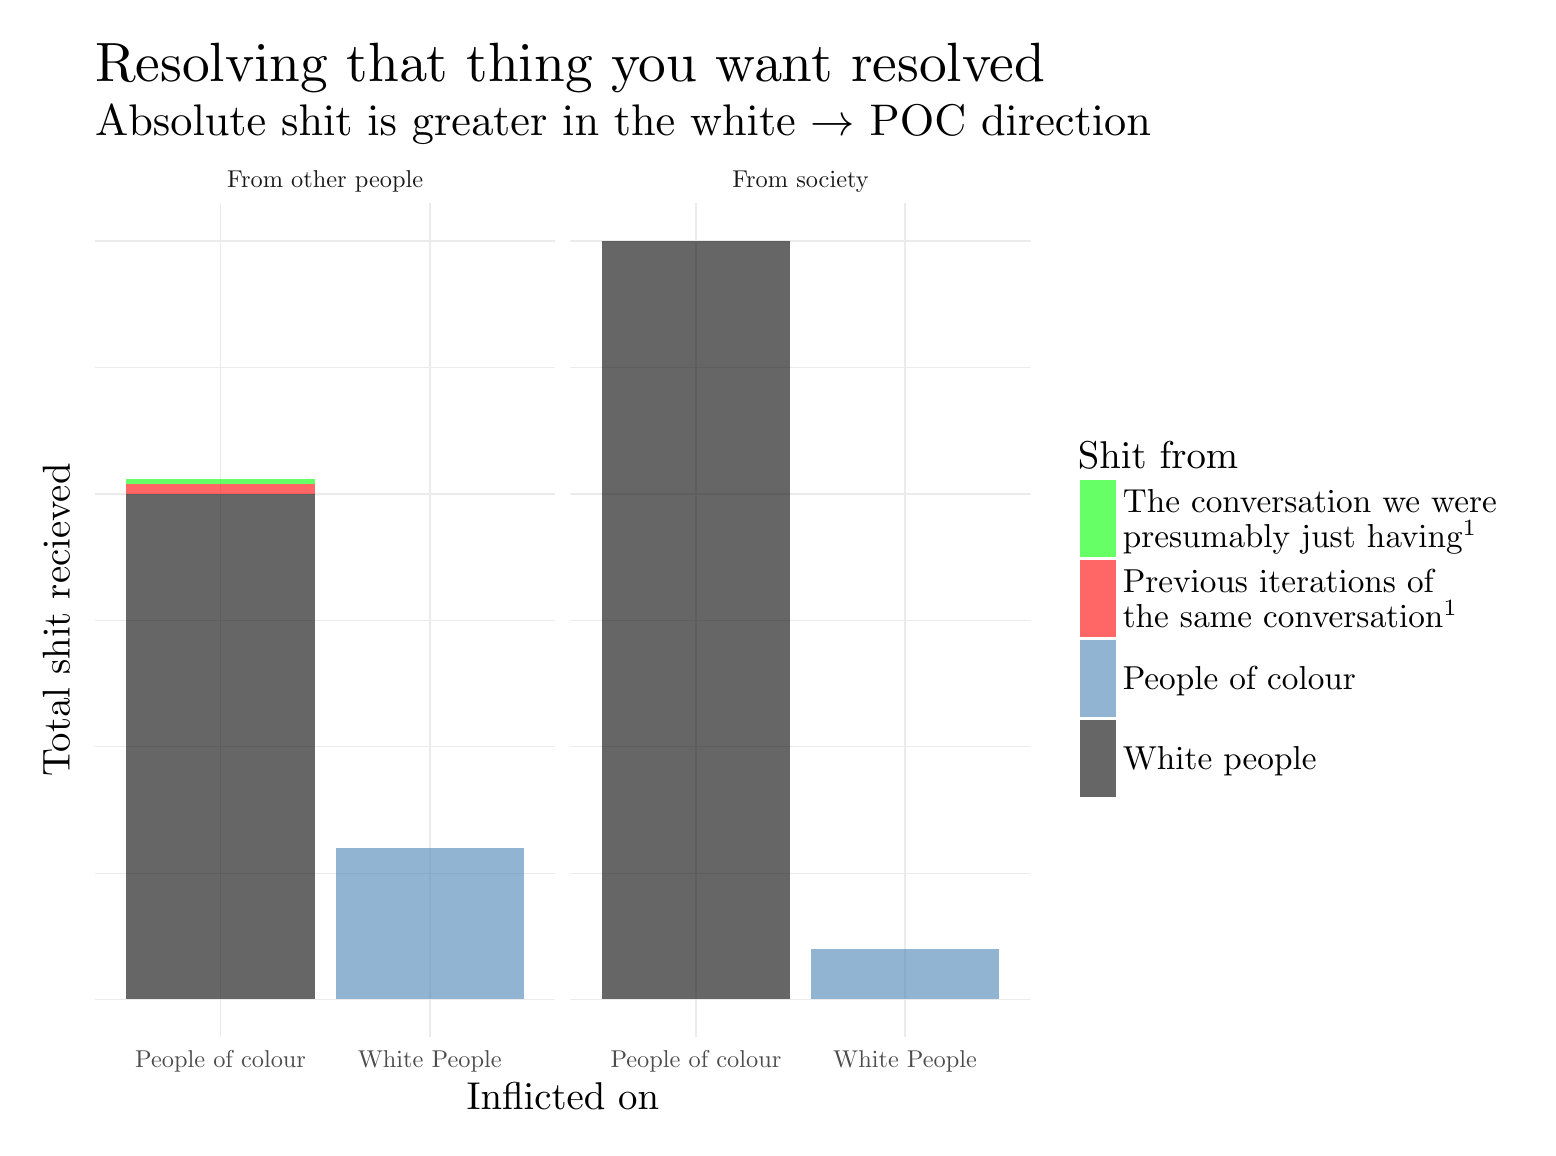
\begin{tikzpicture}[x=1pt,y=1pt]
\definecolor{fillColor}{RGB}{255,255,255}
\path[use as bounding box,fill=fillColor,fill opacity=0.00] (0,0) rectangle (542.02,397.48);
\begin{scope}
\path[clip] ( 24.36, 32.62) rectangle (190.63,334.14);
\definecolor{drawColor}{gray}{0.92}

\path[draw=drawColor,line width= 0.3pt,line join=round] ( 24.36, 92.01) --
	(190.63, 92.01);

\path[draw=drawColor,line width= 0.3pt,line join=round] ( 24.36,183.38) --
	(190.63,183.38);

\path[draw=drawColor,line width= 0.3pt,line join=round] ( 24.36,274.75) --
	(190.63,274.75);

\path[draw=drawColor,line width= 0.6pt,line join=round] ( 24.36, 46.33) --
	(190.63, 46.33);

\path[draw=drawColor,line width= 0.6pt,line join=round] ( 24.36,137.70) --
	(190.63,137.70);

\path[draw=drawColor,line width= 0.6pt,line join=round] ( 24.36,229.06) --
	(190.63,229.06);

\path[draw=drawColor,line width= 0.6pt,line join=round] ( 24.36,320.43) --
	(190.63,320.43);

\path[draw=drawColor,line width= 0.6pt,line join=round] ( 69.71, 32.62) --
	( 69.71,334.14);

\path[draw=drawColor,line width= 0.6pt,line join=round] (145.29, 32.62) --
	(145.29,334.14);
\definecolor{fillColor}{RGB}{0,0,0}

\path[fill=fillColor,fill opacity=0.60] ( 35.70, 46.33) rectangle (103.72,229.06);
\definecolor{fillColor}{RGB}{255,0,0}

\path[fill=fillColor,fill opacity=0.60] ( 35.70,229.06) rectangle (103.72,232.72);
\definecolor{fillColor}{RGB}{0,255,0}

\path[fill=fillColor,fill opacity=0.60] ( 35.70,232.72) rectangle (103.72,234.55);
\definecolor{fillColor}{RGB}{70,130,180}

\path[fill=fillColor,fill opacity=0.60] (111.28, 46.33) rectangle (179.30,101.15);
\end{scope}
\begin{scope}
\path[clip] (196.13, 32.62) rectangle (362.40,334.14);
\definecolor{drawColor}{gray}{0.92}

\path[draw=drawColor,line width= 0.3pt,line join=round] (196.13, 92.01) --
	(362.40, 92.01);

\path[draw=drawColor,line width= 0.3pt,line join=round] (196.13,183.38) --
	(362.40,183.38);

\path[draw=drawColor,line width= 0.3pt,line join=round] (196.13,274.75) --
	(362.40,274.75);

\path[draw=drawColor,line width= 0.6pt,line join=round] (196.13, 46.33) --
	(362.40, 46.33);

\path[draw=drawColor,line width= 0.6pt,line join=round] (196.13,137.70) --
	(362.40,137.70);

\path[draw=drawColor,line width= 0.6pt,line join=round] (196.13,229.06) --
	(362.40,229.06);

\path[draw=drawColor,line width= 0.6pt,line join=round] (196.13,320.43) --
	(362.40,320.43);

\path[draw=drawColor,line width= 0.6pt,line join=round] (241.48, 32.62) --
	(241.48,334.14);

\path[draw=drawColor,line width= 0.6pt,line join=round] (317.06, 32.62) --
	(317.06,334.14);
\definecolor{fillColor}{RGB}{0,0,0}

\path[fill=fillColor,fill opacity=0.60] (207.47, 46.33) rectangle (275.49,320.43);
\definecolor{fillColor}{RGB}{70,130,180}

\path[fill=fillColor,fill opacity=0.60] (283.05, 46.33) rectangle (351.07, 64.60);
\end{scope}
\begin{scope}
\path[clip] ( 24.36,334.14) rectangle (190.63,351.20);
\definecolor{drawColor}{gray}{0.10}

\node[text=drawColor,anchor=base,inner sep=0pt, outer sep=0pt, scale=  0.88] at (107.50,339.64) {From other people};
\end{scope}
\begin{scope}
\path[clip] (196.13,334.14) rectangle (362.40,351.20);
\definecolor{drawColor}{gray}{0.10}

\node[text=drawColor,anchor=base,inner sep=0pt, outer sep=0pt, scale=  0.88] at (279.27,339.64) {From society};
\end{scope}
\begin{scope}
\path[clip] (  0.00,  0.00) rectangle (542.02,397.48);
\definecolor{drawColor}{gray}{0.30}

\node[text=drawColor,anchor=base,inner sep=0pt, outer sep=0pt, scale=  0.88] at ( 69.71, 21.61) {People of colour};

\node[text=drawColor,anchor=base,inner sep=0pt, outer sep=0pt, scale=  0.88] at (145.29, 21.61) {White People};
\end{scope}
\begin{scope}
\path[clip] (  0.00,  0.00) rectangle (542.02,397.48);
\definecolor{drawColor}{gray}{0.30}

\node[text=drawColor,anchor=base,inner sep=0pt, outer sep=0pt, scale=  0.88] at (241.48, 21.61) {People of colour};

\node[text=drawColor,anchor=base,inner sep=0pt, outer sep=0pt, scale=  0.88] at (317.06, 21.61) {White People};
\end{scope}
\begin{scope}
\path[clip] (  0.00,  0.00) rectangle (542.02,397.48);
\definecolor{drawColor}{RGB}{0,0,0}

\node[text=drawColor,anchor=base,inner sep=0pt, outer sep=0pt, scale=  1.40] at (193.38,  6.47) {Inflicted on};
\end{scope}
\begin{scope}
\path[clip] (  0.00,  0.00) rectangle (542.02,397.48);
\definecolor{drawColor}{RGB}{0,0,0}

\node[text=drawColor,rotate= 90.00,anchor=base,inner sep=0pt, outer sep=0pt, scale=  1.40] at ( 15.14,183.38) {Total shit recieved};
\end{scope}
\begin{scope}
\path[clip] (  0.00,  0.00) rectangle (542.02,397.48);
\definecolor{drawColor}{RGB}{0,0,0}

\node[text=drawColor,anchor=base west,inner sep=0pt, outer sep=0pt, scale=  1.40] at (379.47,238.18) {Shit from};
\end{scope}
\begin{scope}
\path[clip] (  0.00,  0.00) rectangle (542.02,397.48);
\definecolor{fillColor}{RGB}{0,255,0}

\path[fill=fillColor,fill opacity=0.60] (380.19,206.37) rectangle (393.22,233.86);
\end{scope}
\begin{scope}
\path[clip] (  0.00,  0.00) rectangle (542.02,397.48);
\definecolor{fillColor}{RGB}{255,0,0}

\path[fill=fillColor,fill opacity=0.60] (380.19,177.46) rectangle (393.22,204.95);
\end{scope}
\begin{scope}
\path[clip] (  0.00,  0.00) rectangle (542.02,397.48);
\definecolor{fillColor}{RGB}{70,130,180}

\path[fill=fillColor,fill opacity=0.60] (380.19,148.56) rectangle (393.22,176.04);
\end{scope}
\begin{scope}
\path[clip] (  0.00,  0.00) rectangle (542.02,397.48);
\definecolor{fillColor}{RGB}{0,0,0}

\path[fill=fillColor,fill opacity=0.60] (380.19,119.65) rectangle (393.22,147.13);
\end{scope}
\begin{scope}
\path[clip] (  0.00,  0.00) rectangle (542.02,397.48);
\definecolor{drawColor}{RGB}{0,0,0}

\node[text=drawColor,anchor=base west,inner sep=0pt, outer sep=0pt, scale=  1.20] at (395.73,222.46) {The conversation we were};

\node[text=drawColor,anchor=base west,inner sep=0pt, outer sep=0pt, scale=  1.20] at (395.73,209.50) {presumably just having$^1$};
\end{scope}
\begin{scope}
\path[clip] (  0.00,  0.00) rectangle (542.02,397.48);
\definecolor{drawColor}{RGB}{0,0,0}

\node[text=drawColor,anchor=base west,inner sep=0pt, outer sep=0pt, scale=  1.20] at (395.73,193.55) {Previous iterations of};

\node[text=drawColor,anchor=base west,inner sep=0pt, outer sep=0pt, scale=  1.20] at (395.73,180.59) {the same conversation$^1$};
\end{scope}
\begin{scope}
\path[clip] (  0.00,  0.00) rectangle (542.02,397.48);
\definecolor{drawColor}{RGB}{0,0,0}

\node[text=drawColor,anchor=base west,inner sep=0pt, outer sep=0pt, scale=  1.20] at (395.73,158.17) {People of colour};
\end{scope}
\begin{scope}
\path[clip] (  0.00,  0.00) rectangle (542.02,397.48);
\definecolor{drawColor}{RGB}{0,0,0}

\node[text=drawColor,anchor=base west,inner sep=0pt, outer sep=0pt, scale=  1.20] at (395.73,129.26) {White people};
\end{scope}
\begin{scope}
\path[clip] (  0.00,  0.00) rectangle (542.02,397.48);
\definecolor{drawColor}{RGB}{0,0,0}

\node[text=drawColor,anchor=base west,inner sep=0pt, outer sep=0pt, scale=  1.60] at ( 24.36,358.65) {Absolute shit is greater in the white $\rightarrow$ POC direction};
\end{scope}
\begin{scope}
\path[clip] (  0.00,  0.00) rectangle (542.02,397.48);
\definecolor{drawColor}{RGB}{0,0,0}

\node[text=drawColor,anchor=base west,inner sep=0pt, outer sep=0pt, scale=  2.00] at ( 24.36,378.21) {Resolving that thing you want resolved};
\end{scope}
\end{tikzpicture}
